%%%%%%%%%%%%%%%%%%%%%%%%%%%%%%%%%%%%%%%%%%%%%%%%%%%%%%%%%%%%%%%%%%%%%%%%%%%%%%%%%%%
% THE BEER-WARE LICENSE (Revision 42): %
% <r@twopi.eu> schrieb diese Datei. Solange Sie diesen Vermerk nicht entfernen, %
% können Sie mit dem Material machen, was Sie möchten. Wenn wir uns eines Tages %
% treffen und Sie denken, das Material ist es wert, können Sie mir dafür ein Bier %
% ausgeben. Robert Hemstedt %
%%%%%%%%%%%%%%%%%%%%%%%%%%%%%%%%%%%%%%%%%%%%%%%%%%%%%%%%%%%%%%%%%%%%%%%%%%%%%%%%%%%

\documentclass[12pt,a4paper]{article}
\usepackage[utf8x]{inputenc}
%\usepackage{ucs}
\usepackage[left=2.0cm, right=2.0cm, top=2.0cm, bottom=2.0cm]{geometry}
\usepackage{amsmath}
\usepackage{amsfonts}
\usepackage[ngerman]{babel}
\usepackage{bbm}
\usepackage{amssymb}
\usepackage[amsthm,thmmarks]{ntheorem}
%\usepackage{tabularx}
\usepackage[arrow, matrix, curve]{xy}
\usepackage{graphicx}
\usepackage{wrapfig}
\usepackage{color}
% b) Lemma, Satz, Theorem usw.
\makeatletter
\renewtheoremstyle{plain}%
  {\item[\hskip\labelsep \theorem@headerfont ##1\ ##2:]}%
  {\item[\hskip\labelsep \theorem@headerfont ##1~##2~##3:]\mbox{}}
\makeatother

\theoremstyle{plain}
\newtheorem{Theorem}{Theorem}[section]
\newtheorem{Satz}[Theorem]{Satz}
\newtheorem{Prop}[Theorem]{Proposition}
\newtheorem{Lemma}[Theorem]{Lemma}
\newtheorem{Korollar}[Theorem]{Korollar}
\newtheorem{Definition}[Theorem]{Definition}
\newtheorem*{Folgerung}[Theorem]{Folgerung}
\newtheorem*{Behauptung}[Theorem]{Behauptung}
\newtheorem{bez}[Theorem]{Bezeichnung}

\theorembodyfont{\upshape}
\newtheorem{Bemerkung}[Theorem]{Bemerkung}
\newtheorem{Beispiel}[Theorem]{Beispiel}

\newcommand{\herv}[1]{{\emph{\textbf{#1}}}}
\newcommand{\N}{\mathbb{N}}
\newcommand{\R}{\mathbb{R}}
\newcommand{\Z}{\mathbb{Z}}
\newcommand{\Q}{\mathbb{Q}}
\newcommand{\C}{\mathbb{C}}
\newcommand{\Ch}{\hat{\C}}
\newcommand{\cupdot}{\mathbin{\dot{\cup}}}

\def\presuper#1#2%
  {\mathop{}%
   \mathopen{\vphantom{#2}}^{#1}%
   \kern-\scriptspace%
   #2}

\numberwithin{equation}{section}

\newsavebox{\fmbox}
\newenvironment{fmpage}[1]
{\begin{lrbox}{\fmbox}\begin{minipage}{#1}}
{\end{minipage}\end{lrbox}\fbox{\usebox{\fmbox}}}

\linespread{1.05}
\author{Robert Hemstedt \\ \texttt{r@twopi.eu}}
\title{Seminarvortrag Verzweigte Überlagerungen Riemannscher Flächen}
\begin{document}
\maketitle
\section{Motivation und weitere Grundlagen}
Wir interessieren uns weiter für holomorphe Abbildungen zwischen Riemannschen Flächen und zeigen mittels der Theorie verzweigter Überlagerungen auf, wie Überlagerungen mit gegebener Decktransformationsgruppe erzeugt werden können. Ebenso knüpfen wir an die unverzweigten Überlagerungen an und setzen sie zu verzweigten Überlagerungen fort und untersuche sie auf einige Eigenschaften.

Überlagerungen Riemannscher Flächen werden etwas anders definiert als topologische Über\-la\-ge\-run\-gen.
\begin{Definition} Eine Abbildung $\eta: X \rightarrow Y$ zwischen Riemannschen Flächen heißt eine \herv{Überlagerung}, wenn für alle $b\in Y\ \exists$ Umgebung $V$, sodass sie \herv{elementar überlagert} wird, d.h. das Urbild $\eta^{-1}(V)$ ist eine Vereinigung von Scheiben $(U,a)$, für welche $\eta|(U,a): (U,a) \rightarrow (V,b)$ Windungsabbildungen sind.
\end{Definition}
\begin{Bemerkung} Die topologische, \emph{unverzweigte} Überlagerung zwischen Riemannschen Flä\-chen erweist sich als Spezialfall, falls die Windungsabbildungen allesamt der Ordnung $1$, also damit biholomorph sind. Damit besitzt sie keine Verzweigungspunkte.
\end{Bemerkung}
Wir erinnern an die 
\begin{Definition}[Deckgruppe] Die \herv{Deckgruppe} $\mathcal{D}(\eta)$ einer Überlagerung (eigentlich sogar jeder holomorphen Abbildung) $\eta: X \rightarrow Y$ zwischen Riemannschen Flächen ist definiert als $\mathcal{D}(\eta) = \{ \varphi: X\rightarrow X \text{ biholomorph }|\eta\circ\varphi = \eta \}$.
\end{Definition}
%\begin{Bemerkung} Falls $X$ und $Y$ in der obigen Definition zusammenhängend sind, ist die Standgruppe $\mathcal{D}(\eta)_a$ endlich (sogar zyklisch) für $a\in X$.
%\end{Bemerkung}
\begin{Definition}Eine surjektive, offene, holomorphe Abbildung $\eta : X \rightarrow Y$ zwischen zusammenhängenden Flächen heißt \herv{normal}, wenn jede Faser ein Orbit (eine Bahn) der Deckgruppe $\mathcal{D(\eta)}$ ist. Normale Abbildungen mit zyklischer Deckgruppe heißen \herv{zyklisch}.
\end{Definition}
Beispiele zyklischer Überlagerungen sind $\C\rightarrow \C, z\mapsto z^n$ oder $\C\rightarrow \C^\times, z\mapsto e^{i z}$. Normal, aber nicht zyklisch ist die Torusprojektion $\C\rightarrow \C/\Omega$ mit dem Gitter $\Omega$.
\begin{Bemerkung} Eine normale Abbildung ist genau dann eine unverzweigte Überlagerung, wenn $\mathcal{D}(\eta)$ frei auf jeder Faser operiert, die Standgruppen der Elemente von $\eta^{-1}$ also trivial sind.
\end{Bemerkung}
%Wir führen \emph{Divisoren} auf Riemannschen Flächen ein:
%\begin{Definition} Ein Divisor auf der Fläche $X$ ist eine Funktion $D: X \rightarrow \Z$, deren Träger $Tr(D):= \{x\in X : D(x) \neq 0\}$ lokal endlich ist. Man nennt dann \begin{enumerate}
%\item $\operatorname{gr} D :=\sum_{x\in X} D(x)$ den \herv{Grad des Divisors}. Zu jeder meromorphen Funktion $f$ , die nirgends konstant Null ist, gehört der Hauptdivisor $(f)$ mit
%\item $(f): X\rightarrow Z ,\ x \mapsto o(f,x)$ .
%\end{enumerate}
%\end{Definition}
%\begin{Bemerkung} Jeder Divisor $D$ auf $\Ch$ vom Grade Null ist Hauptdivisor der rationalen Funktion $\prod_{a\in \C} (z-a)^{D(a)}$. Dies liegt daran, dass für Polynome $p$ $(p)(\infty) = -\operatorname{gr} p$, $p$ als meromorphe Funktion auf $\Ch$ aufgefasst, gilt.
%\end{Bemerkung}

\section{Endliche Automorphismengruppen der Zahlenkugel $\hat{\C}$}
Zunächst klassifizieren wir alle endlichen Automorphismengruppen (bis auf Konjugation) von $\operatorname{Aut}(\hat{\C})$. Später werden wir diese nutzen, um Riemannsche Räume zu konstruieren, die von $\Ch$ und einer entsprechend konstruierten Abbildung mit gewählter Automorphismengruppe überlagert werden.

\begin{Satz} Die Automorphismen auf $\Ch$ sind von der Form \[ z\mapsto A(z):=\frac{az+b}{cz+d},\qquad A=\begin{pmatrix}
a & b \\ c & d
\end{pmatrix} \in \operatorname{GL}_2(\C). \] Man nennt sie Möbius-Transformationen. Eine Möbiustransformation $\neq \operatorname{id}$ hat entweder $2$ oder $3$ Fixpunkte. Möbiustransformationen $g$ mit drei Fixpunkten sind unendlicher Ordnung, d.h. $g^n = \underbrace{g\circ  \ldots \circ g}_{n\text{-mal}} \neq \operatorname{id}$ für $n \geq 1$. 

Die so definierte Abbildung $\operatorname{GL}_2(\C) \rightarrow \operatorname{Aut}(\Ch)$ ist ein Epimorphismus mit Kern $\{\lambda\cdot \mathbbm{1}, \lambda \in \C^\times\}$.
\end{Satz}
\begin{Satz} Jede zyklische Gruppe $G < \operatorname{Aut}(\Ch)$ der Ordnung $n < \infty$ ist zu $C_n := \{z \rightarrow \omega z : \omega\in\mu_n \}$ konjugiert. Diese Gruppe hat zwei Ausnahmebahnen $\{0\}$ und $\{\infty\}$. 
\end{Satz}
%Die Funktion $\Ch \rightarrow \Ch, z\rightarrow z^n$ , ist eine $C_n$-Orbitprojektion.
\begin{proof} Durch Konjugieren erreicht man, dass $G$ durch ein Element $g$ mit
den beiden Fixpunkten $0$ und $\infty$ erzeugt wird. Es folgt $g(z) = \omega z$, wobei
$\omega$ die Gruppe $\mu_n$ der $n$-ten Einheitswurzel erzeugt. 
\end{proof}
\begin{Satz}
Jede nicht-zyklische, endliche Gruppe $G < \operatorname{Aut}(\Ch)$ der Ordnung $N$ hat genau drei Ausnahmeorbiten $\Sigma_1,\Sigma_2,\Sigma_3$. Für deren Mächtigkeiten $s_j :=\sharp\Sigma_j \geq 1$ und für die Ordnungen $n_j:=N/s_j$ der Standgruppen $G_a$ von $a\in \Sigma_j$ gibt es höchstens folgende Möglichkeiten: \begin{center}
\begin{tabular}{|c|c|c|c|c|c|c|c|} \hline
Typ & $N$ & $s_1$ & $s_2$ & $s_3$ & $n_1$ & $n_2$ & $n_3$ \\\hline
$q$-Dieder, $q\geq 2$ & $2q$ & $q$ & $q$ & $2$ & $2$ & $2$ & $q$ \\\hline
Tetraeder & $12$ & $6$ & $4$ & $4$ & $2$ & $3$ & $3$ \\\hline
Oktaeder & $24$ & $12$ & $8$ & $6$ & $2$ & $3$ & $4$ \\\hline
Ikosaeder & $60$ & $30$ & $20$ & $12$ & $2$ & $3$ & $5$ \\\hline
\end{tabular}
\end{center}
Sei $g_j$ ein erzeugendes Element der Standgruppe von $a_j \in \Sigma_j$. Dann wird $G$ von $\{g_1, g_2, g_3\}$ erzeugt. 
%Zwei Gruppen desselben Typs sind in $\operatorname{Aut}(\Ch)$ zueinander konjugiert.
\end{Satz}
Wir konstruieren uns einen Weg, wie wir uns für jede der Gruppentypen eine Gruppe visuell darstellen können. Dazu bemerken wir
\begin{Bemerkung} Durch die stereographische Projektion $\pi:S^2\rightarrow \Ch$ wird die Gruppe $\operatorname{SO_3(\R)}$ zu einer Untergruppe von $\operatorname{Aut}(\Ch)$ gemacht. Dabei sei $\R^3$ als euklidischer Vektorraum mit dem Standardskalarprodukt und seiner induzierten Metrik versehen. Diese Metrik induzieren wir auf die Einheitssphäre und übertragen sie durch $\pi$ nach $\Ch$. Dies ist dann die \emph{chordale Metrik}.
\end{Bemerkung}
\begin{Bemerkung}
Es lässt sich zeigen, dass jede Isometrie auf $\Ch$ bezüglich der chordalen Metrik von der Form $z\mapsto A(z)$ oder $z\mapsto A(\bar{z})$ mit $A\in \operatorname{SU}_2(\C)$, $A(z)$ also eine sogenannte \emph{unitäre} Möbiustransformation ist.
\end{Bemerkung}
Schließlich lässt sich folgender Satz folgern:
\begin{Satz}
Für jedes $T\in\operatorname{SO}_3(\R)$ ist $\varphi:=\pi\circ T\circ\pi^{-1}$ eine unitäre Möbiustransformation. Die Zuordnung $\operatorname{SO}_3(\R) \rightarrow \operatorname{Aut}(\Ch), T\mapsto \varphi$, ist ein Monomorphismus.
\end{Satz}
\begin{proof}
Da $\varphi$ eine Isometrie ist, gibt es nach der obigen Bemerkung ein $A\in\operatorname{SU}_2(\C)$ mit $\varphi(z) = A(z)$ oder $\varphi(z)=A(\bar{z})$. Jedenfalls ist $\varphi^2 = \varphi\circ\varphi$ dann eine Möbiustransformation. Da es zu jedem $A\in\operatorname{SO}_3(\R)$ ein $B\in\operatorname{SO}_3(\R)$ mit $B=A^2$ gibt, ist $\varphi$ eine Möbiustransformation.
\end{proof}
Wir haben nun also eine Möglichkeit gefunden, Drehungen der $S^2$ als Möbius\-trans\-for\-ma\-tio\-nen von $\Ch$ zu verstehen. 
Durch Parkettierungen der $S^2$ lassen sich nun Visualisierungen für die gefunden Automorphismengruppen anschicken.
\begin{figure}[h]
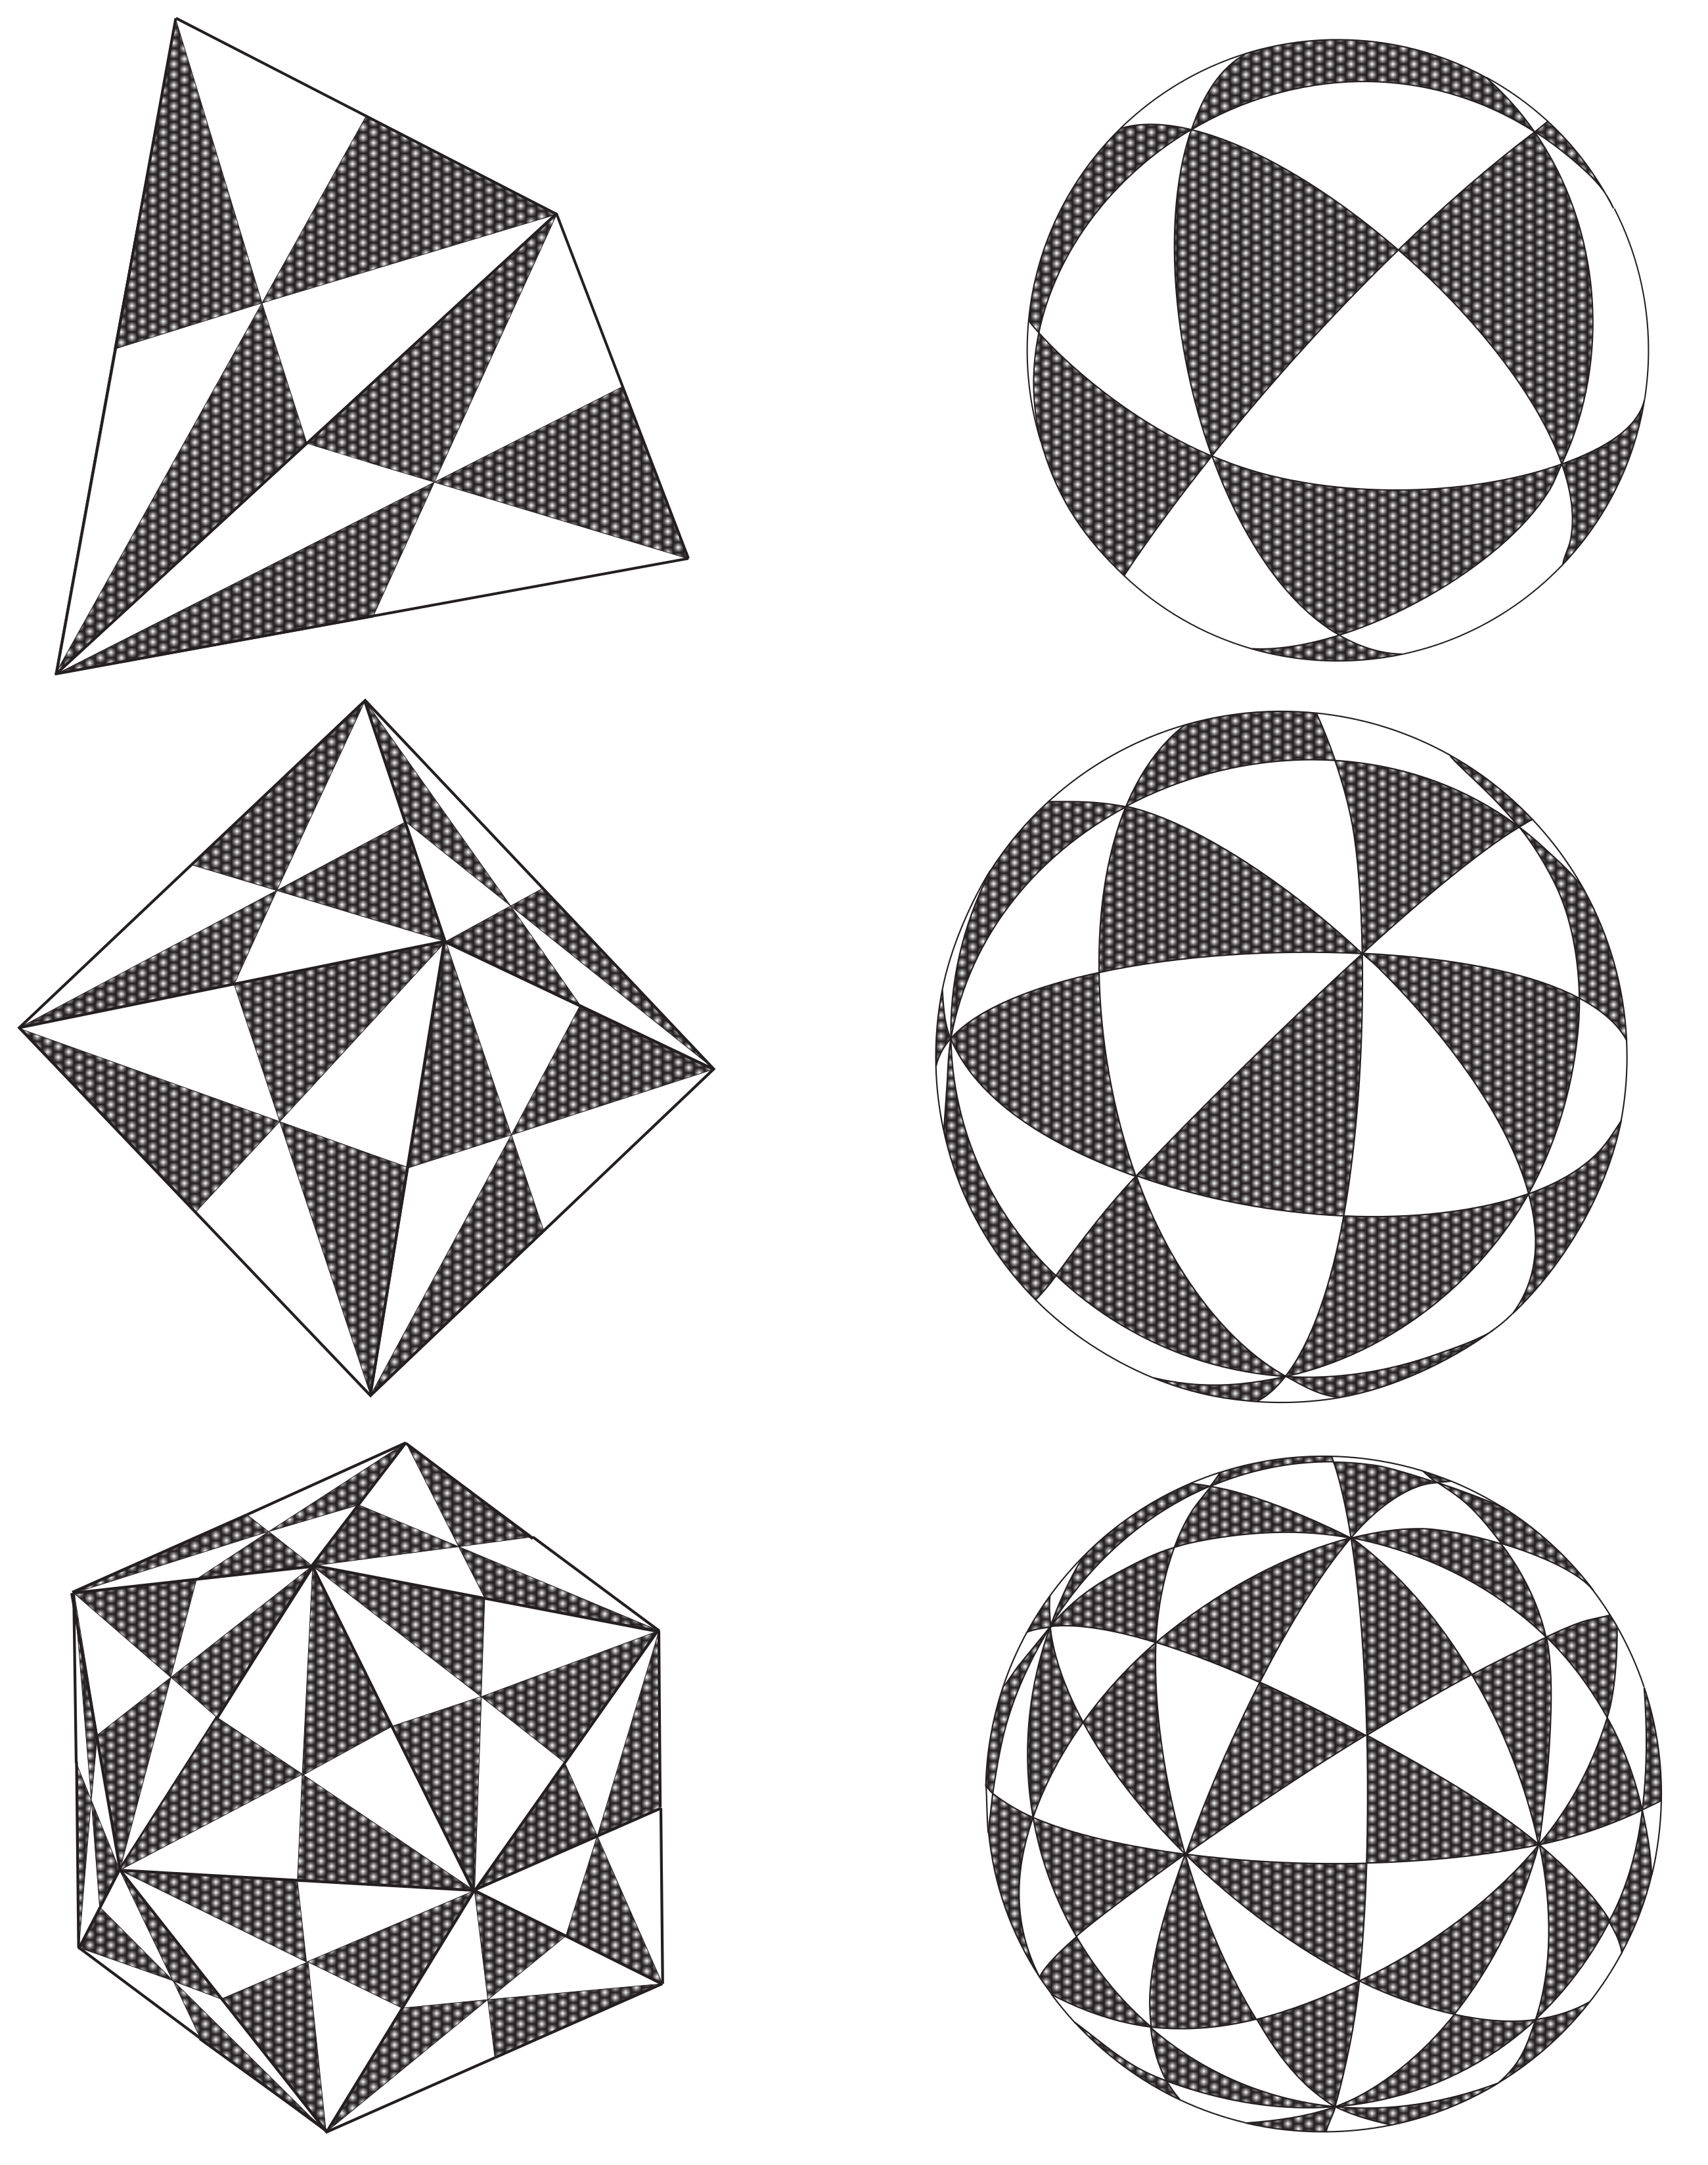
\includegraphics[width=0.8\textwidth]{polyeder.png}
\caption{Linksseitig Parkettierungen des Tetra-, Okta- und Iksoseaders mit Baryzentren jeder Seite. Rechtsseitg die Parkettierungen auf die $S^2$ mittels Radialprojektion übertragen.}
\end{figure}

\noindent Die Automorphismen der Gruppen $G$ sind hierbei für die einzelnen platonischen Körper:
\begin{itemize}
\item \textbf{Tetraeder:} $4$ Achsen durch Ecke/Seitenzentrum mit je $2$, $3$ Achsen durch die Kantenmitten mit je $1$ aus $G\setminus\{\operatorname{id}\}$. Also $4\cdot 2 + 3\cdot 1 + 1 = 12$ Elemente.
\item \textbf{Oktaeder:} $3$ Achsen durch die Ecken mit je $3$, $4$ Achsen durch die Flächenmitten mit je $2$ und $6$ Achsen durch die Kantenmitten mit je $1$ Element aus $G\setminus\{\operatorname{id}\}$. Also $3\cdot 3 + 4\cdot 2 + 6\cdot 1 + 1 = 24$ Elementen.
\item \textbf{Ikosaeder:} $12$ Ecken, $30$ Kanten und $20$ Flächen, das macht analog $6\cdot 4 + 15\cdot 1 + 10\cdot 2 + 1 = 60$.
\end{itemize}

\begin{wrapfigure}{r}{0.5\textwidth} 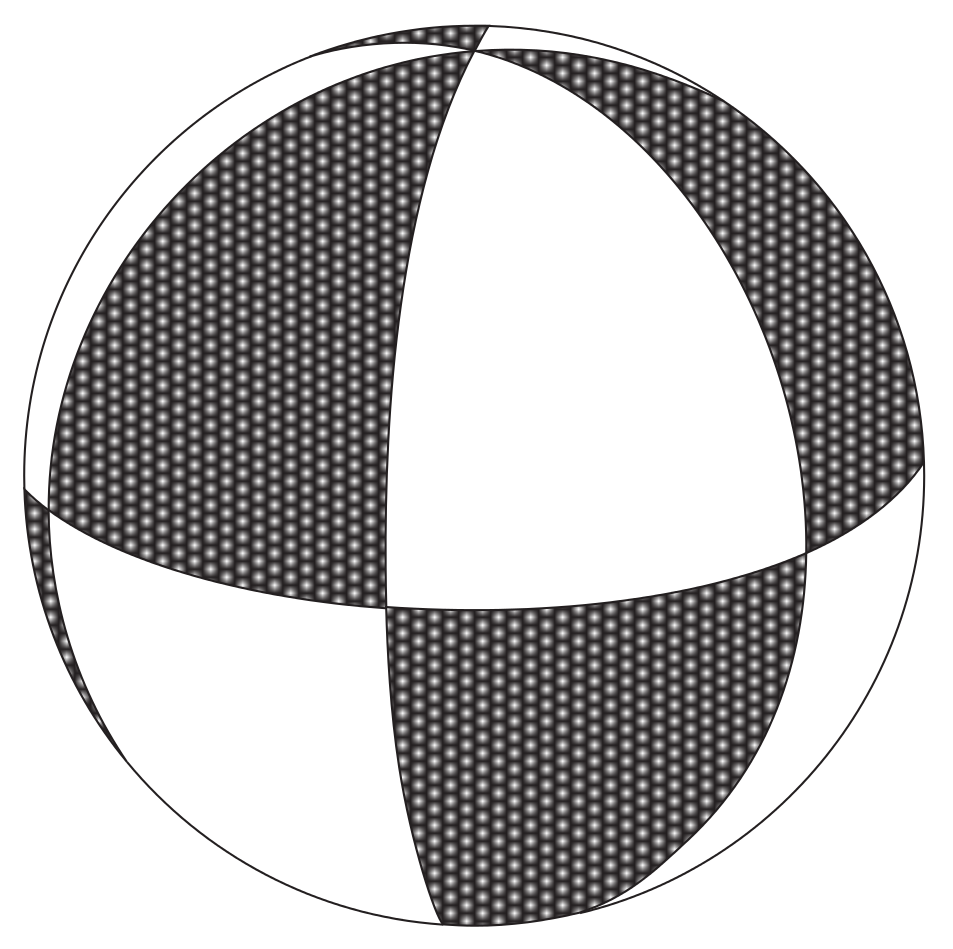
\includegraphics[width=0.5\textwidth]{Dieder.png}
\caption{$3$-Dieder-Parkettierung}
\end{wrapfigure}\noindent Für die $q$-Dieder-Parkettierung haben wir eine $q$-zählige Achse durch den Nord- und Südpol, mit Drehungen um ganzzahlige Vielfache des Winkels $2\pi/q$, sowie $2$ zählige Achsen durch durch die Punkte $A_1,\ldots,A_{2q}$ am Äquator, die die Parkettierung in sich überführen. Diese Drehungen bilden die \emph{orthogonale $q$-Diedergruppe} $D_q$ mit $q-1+q\cdot 1+1=2q$ Elementen. Die Ausnahmeorbiten sind \linebreak $\{\textit{Nordpol}, \textit{Südpol}\}$,$\{A_1,A_3,\ldots,A_{2q-1}\}$ und \linebreak $\{A_2,A_4,\ldots,A_{2q}\}$.

\section{Orbitprojektion und \\Garben}
Wir widmen uns jetzt wieder dem allgemeineren Fall zu, dass wir eine Riemannsche Fläche $X$ und eine Untergruppe $G < \operatorname{Aut}(X)$ gegeben haben. Wir wollen einen Riemannsche Fläche $Y$ und eine Überlagerung $\eta: X\rightarrow Y$ konstruieren mit $\mathcal{D}(\eta) = G$. Dazu definieren wir die
\begin{Definition}[Orbitprojektion] Eine surjektive, stetige, offene Abbildung $\eta:X\rightarrow Y$ zwischen topologischen Räumen, deren Fasern die $G$-Bahnen für $G < \operatorname{Aut}(X)$ sind, heißt \herv{$G$-Orbitprojektion}. Man nennt $Y$ \herv{Orbitraum}.
\end{Definition}

\begin{Satz}[Existenz der Orbitprojektion] Zu jeder Transformationsgruppe $G$ von $X$ existiert eine $G$-Orbitprojektion $\eta:X\rightarrow Y$.
\end{Satz}
\begin{proof}
Sei $Y$ die Menge der $G$-Bahnen. Dann ist $\eta: X\rightarrow Y, x\mapsto G(x)$ surjektiv und wohldefiniert. Definiere auf $Y$ die Quotiententopologie. Wir zeigen noch, dass $\eta$ offen ist: Sei  $U\subset X$ offen, dann ist $g(U)\subset X$ offen für alle $g\in G$. Daher ist $\bigcup_{g\in G} g(U) = \eta^{-1}(\eta(U))\subset X$ offen und damit auch $\eta(U)\subset Y$.
\end{proof}
Man bezeichnet den Raum $Y$ auch mit $X/G$. Beachte, dass aus i.A. aus $X$ hausdorffsch $X/G$ hausdorffsch nicht folgt.

Vergleichen wir nochmal mit der Definition einer normalen Abbildung erhalten wir:
\begin{Satz} Eine holomorphe Abbildung $\eta$ zwischen zusammenhängenden Riemannschen Flächen ist genau dann eine normale Überlagerung, wenn sie eine $\mathcal{D}(\eta)$-Orbitprojektion ist.
\end{Satz}
Wir wollen nun die topologische Orbitprojektion $X\rightarrow X/G$ zu einer holomorphen Abbildung und $X/G$ zu einer Riemannschen Fläche machen, wenn $G<\operatorname{Aut}(X)$. Ab sofort ist $X$ ein \emph{lokal kompakter Hausdorffraum}.
\begin{Definition}[Diskontinuität] Eine Transformationsgruppe $G<\operatorname{Aut}(X)$ heißt \herv{diskontinuierlich}, wenn $\sharp\{g\in G: g(K)\cap K \neq \emptyset \}<\infty$ für alle $K\subset X$ kompakt.
\end{Definition}
Es folgt, dass jede Standgruppe $G_x$ endlich und jede $G$-Bahn lokal endlich ist. -- Endliche Transformationsgruppen sind diskontinuierlich und bei kompakten Räumen $X$ ist umgekehrt jede diskontinuierliche Transformationsgruppe endlich.
\begin{Satz} Der Orbitraum $X/G$ jeder diskontinuierlichen Transformationsgruppe $G$ ist hausdorffsch.
\end{Satz}
\begin{proof}
Sei $\eta: X\rightarrow Y$ eine $G$-Orbitprojektion. Wähle ein Kompaktum $K$ mit $x,y\in \mathring{K}, x\neq y$ und $\eta(x)\neq \eta(y)$. $M:=\{g\in G: g(K)\cap K\neq \emptyset \}<\infty$, da $G$ diskontinuierlich. Da $X$ hausdorffsch und $g\in M$ Automorphismen, gibt es Umgebungen $x\in U$, $y\in V$ mit $g(U)\cap V = \emptyset\ \forall g\in M$. Man kann $U\cup V \subset K$ annehmen (notfalls $U$ und $V$ verkleinern). Dann ist $g(U)\cap V = \emptyset$ \emph{für alle} $g\in G$, weil $g(K)\cap K = \emptyset$ für alle $g\in G\setminus M$. Da $G$ eine Automorphismengruppe ist, folgt insbesondere, dass $g(U)\cap h(V) = \emptyset \ \forall g,h \in G$ und somit $\eta(U) \cap \eta(V) = \emptyset$.
\end{proof}
Später brauchen wir die Eigenschaft einer diskontinuierlichen Gruppe $G$, dass jeder Punkt $a\in X$ eine \emph{privilegierte Umgebung} besitzt:
\begin{Definition} Sei $G$ eine Transformationsgruppe von $X$. Eine Umgebung $U$ von $a\in X$ heißt \herv{privilegiert}, wenn $g(U)=U\ \forall g\in G_a$ und $U \cap g(U) = \emptyset\ \forall g\in G\setminus G_a$. Durch Beschränkung entsteht aus der $G$-Orbitprojektion $\eta:X\rightarrow Y$ die $G_a$-Orbitprojektion $\eta|U : U\rightarrow \eta (U)$.
\end{Definition}
Da $X$ als Riemannsche Fläche hausdorffsch ist, ist $X/G$ hausdorffsch. Bleibt die Frage nach einer holomorphen Struktur auf $X/G$ zu ergründen, die die Orbitprojektion holomorph macht. Dazu führen wir das Konzept der \emph{Garben} ein.

\begin{Definition}Eine \herv{(Funktionen-)Garbe $\mathcal{F}$} auf dem topologischen Raum $X$ ordnet jeder offenen Menge $U\subset X$ einen Ring $\mathcal{F}(U)$ stetiger Funktionen $U\rightarrow \C$ zu, welche alle konstanten Funktionen umfasst und daher eine $\C$-Algebra ist. Dabei wird folgendes \herv{Lokal-Global-Prinzip} verlangt:

Für jede Familie $\{U_j\}$ von offenen Mengen gilt:
\begin{enumerate}
\item Falls $f\in \mathcal{F}(\bigcup U_j)$, dann ist für alle $U_j$: $f|U_j \in \mathcal{F}(U_j)$.
\item Falls es $f_j\in \mathcal{F}(U_j)$ gibt mit: für alle $U_i,U_j \in \{U_l\}$ ist $f_i|U_i\cap U_j \in \mathcal{F}(U_i\cap U_j)$ und $f_j|U_i\cap U_j \in \mathcal{F}(U_i\cap U_j)$ und $f_i|U_i\cap U_j = f_j|U_i\cap U_j$, dann existiert ein eindeutiges $f\in \mathcal{F}(\bigcup U_i)$, so dass $f|U_i = f_i$ für alle $U_i$.
\end{enumerate}
Ein topologischer Raum $X$ zusammen mit einer Garbe $\mathcal{F}$ wird \herv{geringter Raum} $(X,\mathcal{F})$ genannt. Für $U\subset X$ offen bezeichnet $\mathcal{F}|U$ die Einschränkung von $\mathcal{F}$ auf die offenen Teilmengen von $U$. Statt $(U,\mathcal{F}|U)$ schreibe auch $(U,\mathcal{F})$.

Ein \herv{Morphismus} $\varphi:(X,\mathcal{F})\rightarrow (Y,\mathcal{G})$ zwischen geringten Räumen ist eine stetige Abbildung $\varphi:X\rightarrow Y$ mit folgender Eigenschaft: Für alle $V\subset Y$ offen und $\forall g\in \mathcal{G}(V)$ gilt $g\circ\varphi \in \mathcal{F}(\varphi^{-1}(V))$. Hintereinanderschaltung von Morphismen ist ein Morphismus, ein \herv{Isomorphismus} ist bijektiver Morphismus $\varphi$ mit $\varphi^{-1}$ ein Morphismus. Isomorphismen in den gleichen geringten Raum heißen Automorphismen. Sie bilden mit Hintereinanderschaltung die Automorphismengruppe $\operatorname{Aut}(X,\mathcal{F})$.
\end{Definition}

\begin{Definition}\herv{Die holomorphe Strukturgarbe $\mathcal{O}$} einer Riemannschen Fläche $X$ benutzt statt der stetigen Funktionen, die holomorphen Funktionen für seine Definition. Schreibe auch $\mathcal{O}_X$. Die Morphismen $(X,\mathcal{O_X})\rightarrow (Y,\mathcal{O}_Y)$ sind genau die holomorphen Abbildungen.
\end{Definition}
Mithilfe der holomorphen Strukturgarbe haben wir nun eine weitere Möglichkeit, Riemannsche Flächen zu definieren:
\begin{Satz} Ein geringter Hausdorffraum $(X,\mathcal{F})$ ist genau dann eine Riemannsche Fläche, wenn er zu $(\C,\mathcal{O})$ lokal isomorph ist, d.h. für alle $x\in X$ gibt es ein $x\in U\subset X$ offen und $V\subset \C$ offen, so dass $(U,\mathcal{F})$ und $(V,\mathcal{O})$ isomorph sind.
\end{Satz}
\begin{proof}
Bei einer Riemannschen Fläche $(X,\mathcal{F})$ ist jede holomorphe Karte $(U,h)$ ein Isomorphismus $h:(U,\mathcal{F})\rightarrow (h(U),\mathcal{O})$. Wenn umgekehrt $(X,\mathcal{F})$ zu $(\C,\mathcal{O})$ lokal isomorph ist, wird $X$ durch offene Mengen $U_j$ überdeckt, zu denen Isomorphismen $h_j:(U_i,\mathcal{F})\rightarrow (V_j,\mathcal{O})$ auf offene Mengen $V_j\subset\C$ gehören. Dann ist $\{(U_j,h_j)\}$ ein holomorpher Atlas. Die Kartenwechsel sind holomorph, denn: $h_i^{-1}|h_i(U_i\cap U_j) : (h(U_i\cap U_j),\mathcal{O}) \xrightarrow{\cong} (U_i\cap U_j,\mathcal{F})$ Isomorphismus $\Leftrightarrow \forall g: U_i \cap U_j \rightarrow \C$ gilt $g\circ h_i \in \mathcal{O}(h_i(U_i\cap U_j))$, insbesondere für $g=h_j$.
\end{proof}
Wie beim Quotientenprinzip wollen wir die Garbe von $X$ auf den Orbitraum $X/G$ \glqq übertragen\grqq.
\begin{Definition} Sei $(X,\mathcal{F})$ ein geringter Raum und $\eta: X\rightarrow Y$ eine surjektive stetige Abbildung auf einen topologischen Raum $Y$. Mit der Garbe $\mathcal{C}$ der stetigen Funktionen auf $Y$ wird die \herv{Bildgarbe $\mathcal{F}_\eta$} auf $Y$ durch \[\mathcal{F}_\eta(V):=\{f\in\mathcal{C}(V):f\circ\eta\in\mathcal{F}(\eta^{-1}(V))\} \text{ für jede offene Menge }V\subset Y \]
definiert. Das Lokal-Global-Prinzip ist auch hier erfüllt, und $\eta:(X,\mathcal{F})\rightarrow (Y,\mathcal{F}_\eta)$ ist ein Morphismus.
\end{Definition}
Wir sind fast fertig. Wir müssen unseren geringten Hausdorffraum $(Y,\mathcal{F}_\eta)$ jetzt noch zur Riemannschen Fläche werden lassen:
\begin{Satz} Sei $\eta: X\rightarrow Y$ $G$-Orbitprojektion, $G < \operatorname{Aut}(X,\mathcal{F})$ diskontinuierlich. $(Y,\mathcal{F}_\eta)$ ist ein geringter Hausdorffraum. Wenn es zu jedem $a\in X$ eine privilegierte Umgebung $U$ und eine $G_a$-Orbitprojektion $\varphi :U\rightarrow V$ gibt, sodass $(V,\mathcal{F}_\varphi)$ eine Riemannsche Fläche ist, dann ist $(Y,\mathcal{F}_\eta)$ eine Riemannsche Fläche.
\end{Satz}
Glücklicherweise sind die Voraussetzungen dieses Satzes auch tatsächlich gegeben, dies zu beweisen ist aber eher technisch. Damit schließen wir diesen Teil der Untersuchungen von Orbitprojektionen mit  folgendem Satz ab:
\begin{Satz} Bei jeder diskontinuierlichen Automorphismengruppe $G<\operatorname{Aut}(X)$ einer zusammenhängenden Riemannschen Fläche $X$ ist der Orbitraum $(Y,\mathcal{O}_\eta)$ mit der Bildgarbe der $G$-Orbitprojektion $\eta: X\rightarrow Y$ eine Riemannsche Fläche. Die Projektion $\eta$ ist holomorph.
\end{Satz}
\section{Fortsetzung unverzweigter Überlagerungen}
Nachdem wir verzweigte, normale Überlagerungen direkt konstruiert haben, wollen wir einen Blick auf unverzweigte Überlagerungen werfen und sehen, ob sich diese zu verzweigten Über\-la\-ge\-run\-gen fortsetzen lassen.

Für eine lokal endliche Menge $B\subset Y$ einer Riemannschen Fläche Y bezeichnen wir eine Überlagerung $\hat{\eta}:\hat{X} \rightarrow Y$ als Fortsetzung der Überlagerung $\eta: X \rightarrow  Y\setminus B$, wenn $X=\hat{X}\setminus\eta^{-1}(B)$ und $\eta = \hat{\eta}|X$ gelten. Wir zeigen zunächst den
\begin{Satz} Die unendlich-blättrige, unverzweigte Überlagerung $\eta: \mathbb{H}\rightarrow \mathbb{E}^\times$ lässt sich nicht zu einer verzweigten Überlagerung von $\mathbb{E}$ fortsetzen.
\end{Satz}
\begin{proof}
Angenommen, $\eta$ ließe sich fortsetzen. Dann würde eine kleine Scheibe $\mathbb{E}_r$ elementar überlagert werden. Damit wäre für jede Komponente $U$ von $\eta^{-1}(\mathbb{E}_r^\times)$ $\eta|U : U\rightarrow \mathbb{E}_r^\times$ eine endliche Abbildung. Aber bei der Exponentialabbildung ist $\eta^{-1}(\mathbb{E}^\times_r) = U$ zusammenhängend und $\eta|U$ hat unendlich viele Blätter.
\end{proof}
\begin{Satz} Die unverzweigte Überlagerung $\eta: X\rightarrow Y\setminus B$ lässt sich genau dann zu einer Überlagerung $\hat{\eta}: \hat{X} \rightarrow Y$ fortsetzen, wenn jeder Punkt $b\in B$ Zentrum einer Scheibe $V$ ist, so dass für $V^\times:=V\setminus\{b\}$ und jede Komponente $U$ von $\eta^{-1}(V^\times)$ die Beschränkung $\eta|U: U\rightarrow V^\times$ endlich ist. Insbesondere existiert die Fortsetzung für jede endliche Abbildung $\eta$.
\end{Satz}
\begin{figure} \def\svgwidth{\textwidth} \input{KonstrVerzwUe.pdf_tex} \caption{Fortsetzung zur  verzweigten Überlagerung}\label{KVUe}
\end{figure}
\begin{proof}
Die Endlichkeitsbedingung an die Abbildung ist notwendig, wie wir soeben gesehen haben. Konstruiere die Fortsetzung wie folgt:
\begin{itemize}
\item Wähle paarweise disjunkte Scheiben $V\subset Y$ um die Punkte in $b\in B$ und Karten $z:(V,b)\rightarrow (\mathbb{E},0)$.
\item Aus der Endlichkeitsbedingung folgt, dass es zu jeder Komponente $U$ von $\eta^{-1}(V^\times)$ einen Isomorphismus $h: U\rightarrow \mathbb{E}^\times$ mit $z\circ \eta|U = h^n$ gibt, $n$ abhängig von $U$.
\item Ergänze $U$ um Punkt $a_U$ zu $\hat{U}:=U\cupdot a_U$ und ergänze $h$ zur bij. Abbildung $h: (\hat{U},a_U) \rightarrow (\mathbb{E},0)$. Siehe Abb. \ref{KVUe}.
\item $A$ sei die Menge der zusätzlichen Punkte, dann definiere auf $\hat{X} = X \cupdot A$ die folgende Topologie: $W\subset \hat{X}$ offen, wenn $W\cap X \subset X$ offen in $X$ ist und für alle Komponenten $\hat{U}$ aus der Konstruktion die Bilder $h(W\cap \hat{U})\subset \mathbb{E}$ offen in $\mathbb{E}$ sind. Das macht $\hat{X}$ zu einem Hausdorff-Raum, so dass $A\subset \hat{X}$ lokal endlich ist.
\item Ergänze den holomorphen Atlas von $X$ um die Karten $h:\hat{U}\rightarrow \mathbb{E}$ der Konstruktion. Damit wird $\hat{X}$ zu einer Riemannschen Fläche.
\item Definiere $\hat{\eta}: \hat{X}\rightarrow Y$ durch $\hat{\eta}|X = \eta, \hat{\eta}(a_U)=b$ für $b$ Zentrum der Scheibe $V$, für die $U$ eine Komponente von $\eta^{-1}(V^\times)$ ist.
\item Aus der Konstruktion folgt, dass $\hat{\eta}:\hat{X}\rightarrow Y$ die Definition einer Überlagerung erfüllt und $\eta: X\rightarrow Y\setminus B$ fortsetzt.
\end{itemize}
\end{proof} Mit dem
\begin{Lemma} Sei $\eta : X \rightarrow Y$ eine Überlagerung. Sei $Z$ ein bei $c\in Z$ unzerlegbarer Hausdorffraum, d.h. es gibt eine Umgebungsbasis $\{W\}$ von $c$, sodass $W\setminus \{c\}$ zusammenhängt. Dann lässt sich jede stetige Abbildung $\varphi : Z\setminus \{c\} \rightarrow X$ stetig nach $c$ fortsetzen, sobald dies für $\eta\circ\varphi$ gilt. Bei einer Riemannschen
Fläche $Z$ ist mit $\varphi$ auch die Fortsetzung holomorph.
\end{Lemma}
folgt, dass die Fortsetzungen $\hat{X}$ und $\hat{\eta}$ eindeutig sind. Ebenso sind verzweigte Überlagerungen bereits gleich (bis auf Isomorphie), wenn dies für ihre Einschränkung auf die unverzweigte Überlagerung gilt.

Auch wenn die Hintereinanderschaltung zweier verzweigter Überlagerungen i.A. keine Über\-la\-ge\-rung ist, so gilt folgender
\begin{Satz} Ist $\eta: X\rightarrow Y$ eine unverzweigte und $\varphi: Y\rightarrow Z$ eine eventuell verzweigte Überlagerung, dann ist $\zeta:=\varphi\circ \eta$ eine Überlagerung.
\end{Satz}
\section{Universelle verzweigte Überlagerung}
Wir betrachten nur zusammenhängende, holomorphe Überlagerungen $\eta:X\rightarrow Y$ mit beschränkten Windungszahlen längs jeder Faser. Nenne die Überlagerung \emph{einfach zusammenhängend}, falls ihre Überlagerungsfläche $X$ einfach zusammenhängt.
\begin{Definition} Eine Funktion $S:Y\rightarrow \N_{>0}$ heißt \herv{Signatur}, wenn ihr \herv{Träger} $\{y\in Y: S(y) \geq 2 \}$ lokal endlich ist. Die Signatur $S_1$ \herv{teilt} $S$, wenn  für alle $y\in Y$ $S_1(y)|S(y)$ gilt. Zu jeder Überlagerung $\eta:X\rightarrow Y$ definiere die Verzweigungssignatur $S_\eta(y):=\operatorname{kgV}\{v(\eta,x) : x \in \eta^{-1}(y)\}$
\end{Definition}
\begin{Definition} Seien $\eta:X\rightarrow Y$ und $\zeta: Z\rightarrow Y$ Überlagerungen, wenn es eine holomorphe Abbildung $\gamma: Z\rightarrow X$ gibt, mit $\zeta = \eta \rightarrow \gamma$, dann sagen wir, dass $\eta$ durch $\zeta$ \herv{dominiert} wird. 

Aus der Faktorisierung von Überlagerungen geht hervor, dass $\gamma$ auch eine Überlagerung ist und wegen Produktformel der Windungszahlen gilt $S_\eta | S_\zeta$. Nenne $\zeta$ \herv{universell}, wenn $\zeta$ alle Überlagerungen $\eta$ mit $S_\eta | S_\zeta$ dominiert.
\end{Definition}
\end{document}
